\documentclass{article}
\usepackage[utf8]{inputenc}
\usepackage{amsmath}
\usepackage{siunitx}
\usepackage{array}
\usepackage{multirow}
\usepackage{chemfig} 
\usepackage[version=4]{mhchem}
\usepackage[a4paper, total={6.5in, 9in}]{geometry}
\usepackage{graphicx}
\usepackage{setspace}
% \usepackage{hyperref}
\usepackage[super]{nth}
\usepackage{comment}
\graphicspath{{./images}}
\parindent=0pt

\DeclareSIUnit{\mmHg}{mmHg}
\DeclareSIUnit{\bar}{bar}
\DeclareSIUnit{\torr}{torr}
\DeclareSIUnit{\atm}{atm}
\DeclareSIUnit{\Molar}{\textsc{m}}

\onehalfspacing

\title{CHEM 154 Notes}
\author{Raymond Wang}
\date{July 2022}

\begin{document}

% \begin{comment}

\maketitle

\tableofcontents

\section{Atoms, Ions, and Isotopes}

\subsection{Subatomic Particles}

\begin{center}
    \begin{tabular}{|c|c|c|c|}
        \hline
        \textbf{Particle} & \textbf{Mass (\si{\gram})} & \textbf{Mass (amu or \si{\gram\per\mol})} & \textbf{Relative Charge} \\ 
        \hline
        Proton & $1.673 \times 10^{-24}$ & $1.007$ & $+1$ \\  
        Neutron & $1.675 \times 10^{-24}$ & $1.009$ & $0$ \\
        Electron & $9.109 \times 10^{-28}$ & $5.485 \times 10^{-4}$ & $-1$ \\
        \hline 
    \end{tabular}
\end{center}

\subsection{Chemical Symbols and Notation}

\begin{center}
    \ce{^{A}_{Z}X^n}
\end{center}

\begin{itemize}
    \item X: chemical symbol for the element
    \item A: atomic mass = number of protons + neutrons
    \item Z: atomic number = number of protons
    \item n: charge of element
\end{itemize}

\section{Early Atomic Theory to Quantum Theory}

\subsection{Photon Equations}

\begin{equation*}
    E = \frac{hc}{\lambda} = h\nu
\end{equation*}

\begin{itemize}
    \item $E$: energy in \si{\joule}
    \item $h$: Planck's constant = \SI{6.626e-34}{\joule\second}
    \item $c$: speed of light = \SI{3.0e8}{\meter \per \second}
    \item $\lambda$: wavelength in \si{\meter}
    \item $\nu$: frequency in \si{\per\second} or \si{\hertz}
\end{itemize}

\subsection{Bohr Model}

\subsubsection{Energy of a Specific $n$ Level}

\begin{equation*}
    E = \frac{(\SI{-2.178e-18}{\joule})(Z^2)}{n^2}
\end{equation*}

\begin{itemize}
    \item $n$: shell number (1, 2, 3, etc)
    \item $E$: energy of a specific $n$ level in \si{\joule}
    \item $Z$: atomic number
\end{itemize}

\subsubsection{Energy Difference Between $n$ Levels}

\begin{equation*}
    \Delta E = (\SI{-2.178e-18}{\joule})(Z^2) \left(\frac{1}{n_f^2} - \frac{1}{n_i^2}\right)
\end{equation*}

\begin{itemize}
    \item $\Delta E$: difference in energy in \si{\joule}
    \item $n_f$: final energy level
    \item $n_i$: initial energy level
\end{itemize}

\subsubsection{Wavelength of the Photon Absorbed or Emitted}

\begin{equation*}
    \frac{1}{\lambda} = R_h \left(\frac{1}{n_f^2} - \frac{1}{n_i^2}\right)
\end{equation*}

\begin{itemize}
    \item $R_h$: Rydberg's constant = \SI{1.097e7}{\per\meter}
\end{itemize}

\subsubsection{Hydrogen Emission Spectral Series}

\begin{center}
    \begin{tabular}{|c|c|}
        \hline
        \textbf{Hydrogen Emission Spectrum Series Name} & $n_f$ \\ 
        \hline
        Lyman & 1 \\
        Balmer & 2 \\
        Paschen & 3 \\
        Brackett & 4 \\
        Pfund & 5 \\
        \hline 
    \end{tabular}
\end{center}

\section{The Quantum Model and Orbitals}

\subsection{Quantum Numbers}

% \begin{center}
%     \begin{tabular}{|m{10em}|m{10em}|m{10em}|m{10em}|}
%         \hline
%         \textbf{Principle Quantum Number ($n$)} & \textbf{Angular Momentum Quantum Number ($l$)} & \textbf{Magnetic Quantum Number ($m_l$)} & \textbf{Electron-Spin Quantum Number ($m_s$)} \\
%         \hline
%     \end{tabular}
% \end{center}                

\begin{center}
    \begin{tabular}{|c|c|c|}
         \hline
         \textbf{Letter} & \textbf{Quantum Number} & \textbf{Description} \\
         \hline
         $n$ & Principal & Size \\
         $l$ & Orbital Angular Momentum & Shape \\
         $m_l$ & Magnetic & Orientation \\
         $m_s$ & Electronic Spin & Electron Up or Down \\
         \hline
    \end{tabular}
\end{center}

\begin{itemize}
    \item $n$: Can be any positive integer. As $n$ increases, energy and size of the shell increases. Indicates shell.
    \item $l$: Can be any non-negative integer up to $n - 1$. Indicates sub-shell within shell.
    \begin{center}
        \begin{tabular}{|c|c|c|}
            \hline
            \textbf{Sub-shell} & $l$ & Number of electrons \\
            \hline
            s & 0 & 2 \\
            p & 1 & 6 \\
            d & 2 & 10 \\
            f & 3 & 14 \\
            \hline
        \end{tabular}
    \end{center}
    \item $m_l$: Can be any integer from $-l$ to $+l$. Indicates orbital within sub-shell.
    \item $m_s$: Can be $+\frac{1}{2}$ or $-\frac{1}{2}$. Indicates spin of an electron. There are always $2$ electrons per orbital.
\end{itemize}

\subsection{Orbital Shapes}

\begin{center}
    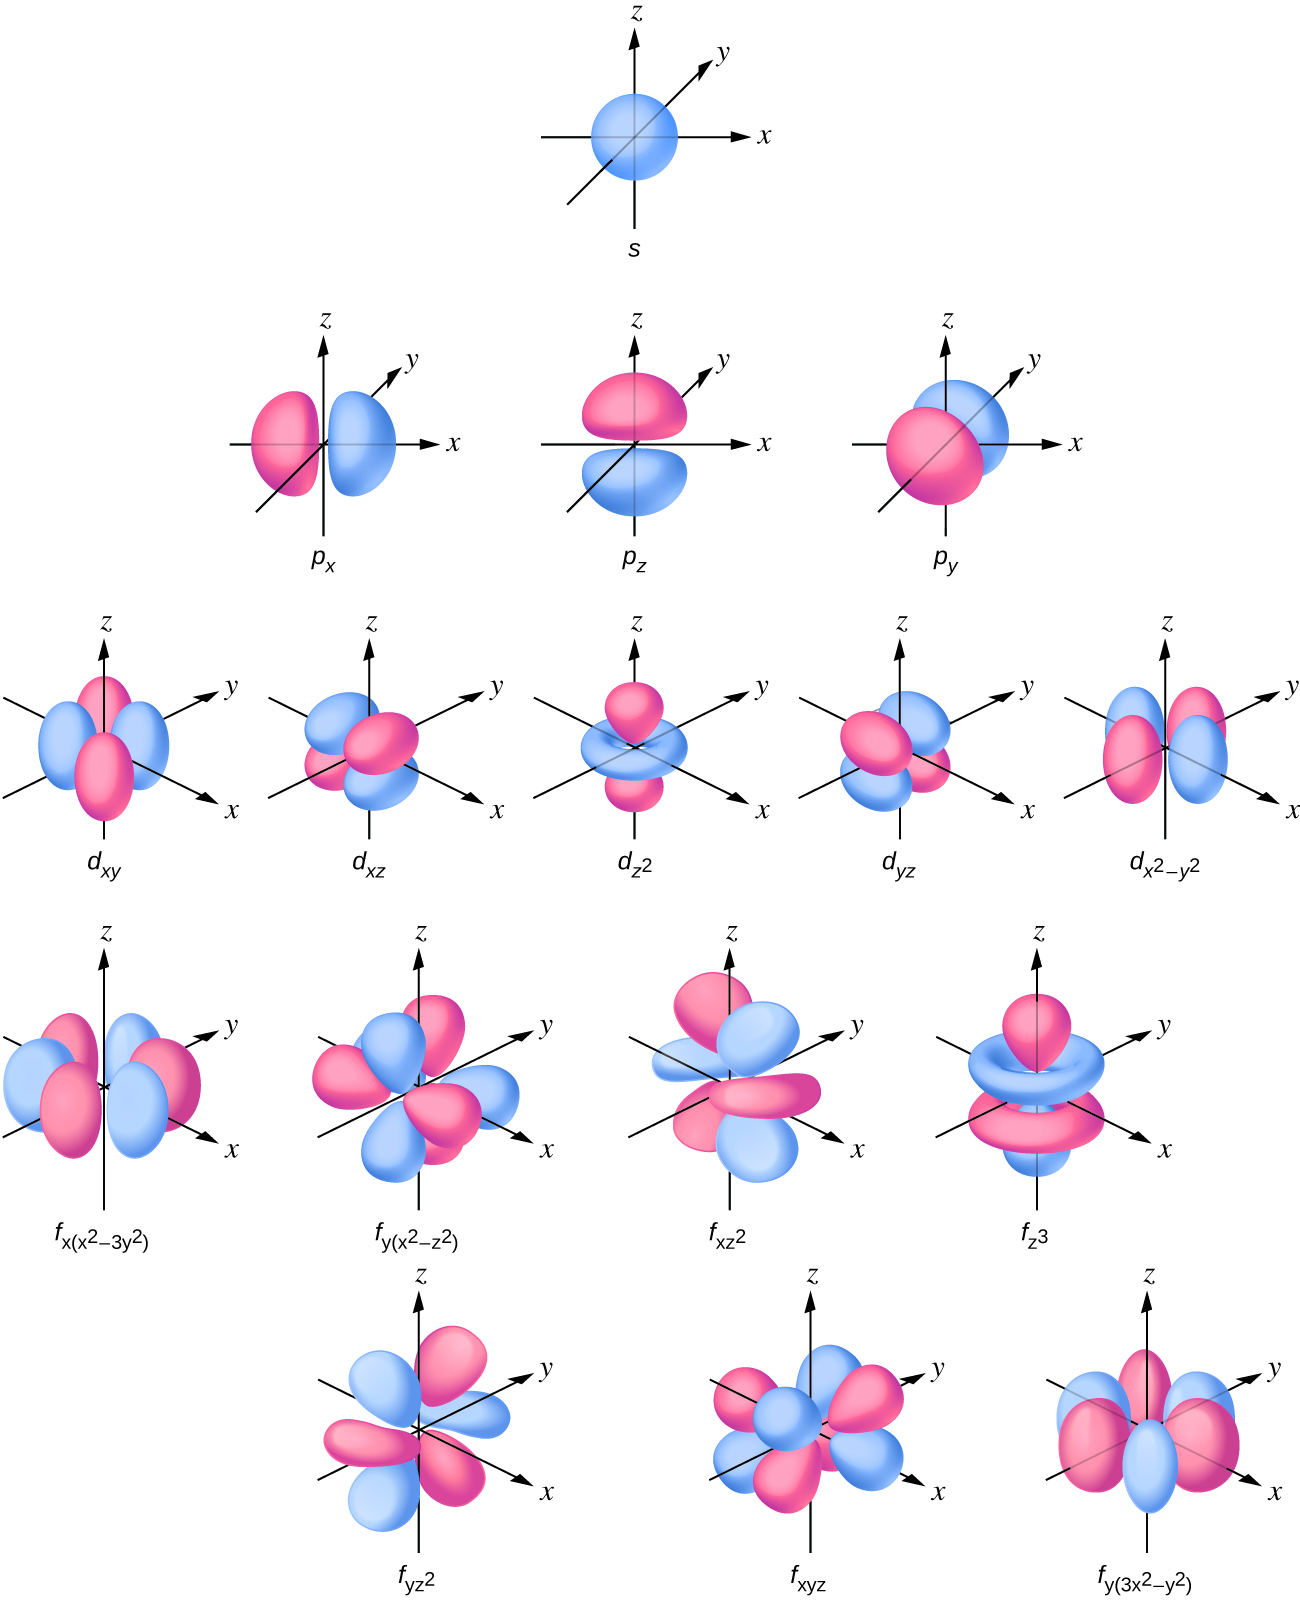
\includegraphics[scale=0.2]{orbital_shapes}
\end{center}

\subsection{Rules for Orbital Filling}

\subsubsection{Aufbau Principle}

\begin{itemize}
    \item Electrons will always occupy the lowest available energy level first.
\end{itemize}

\begin{center}
    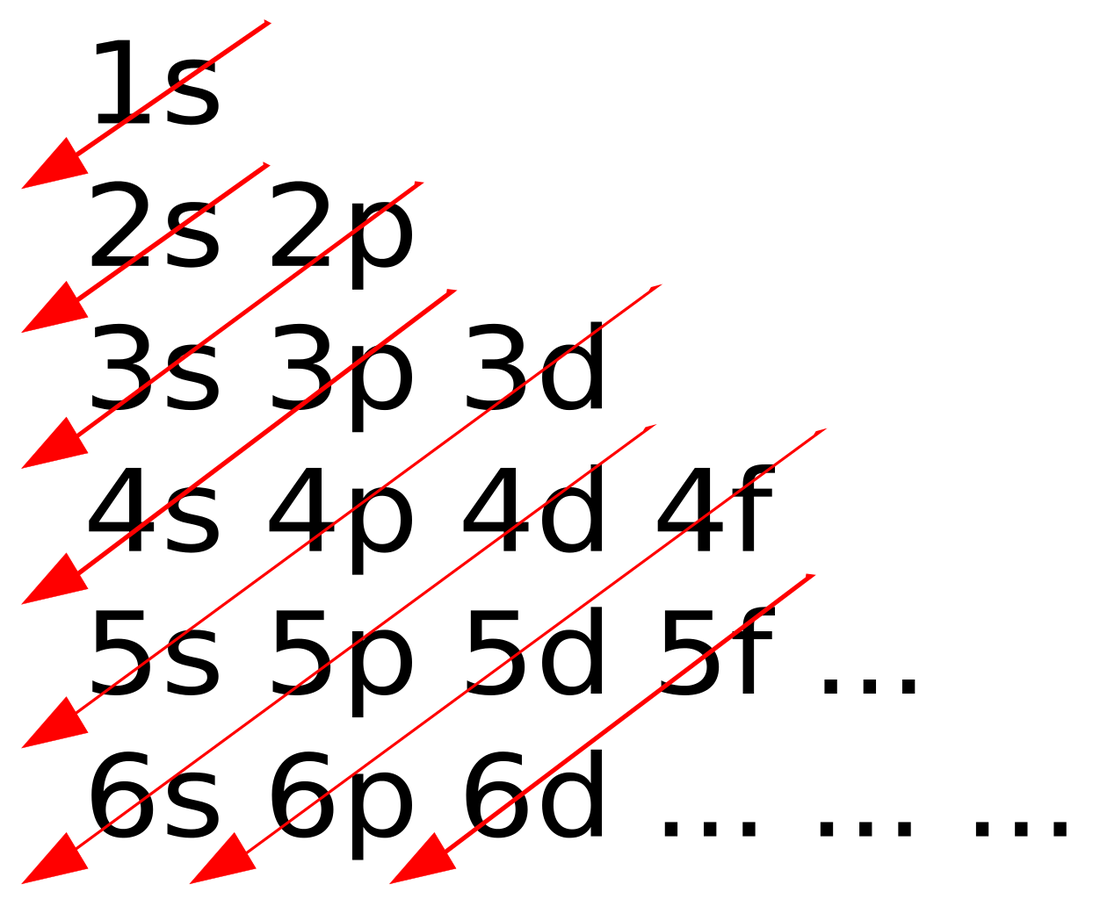
\includegraphics[scale=0.1]{aufbau_principle}
\end{center}

\begin{center}
    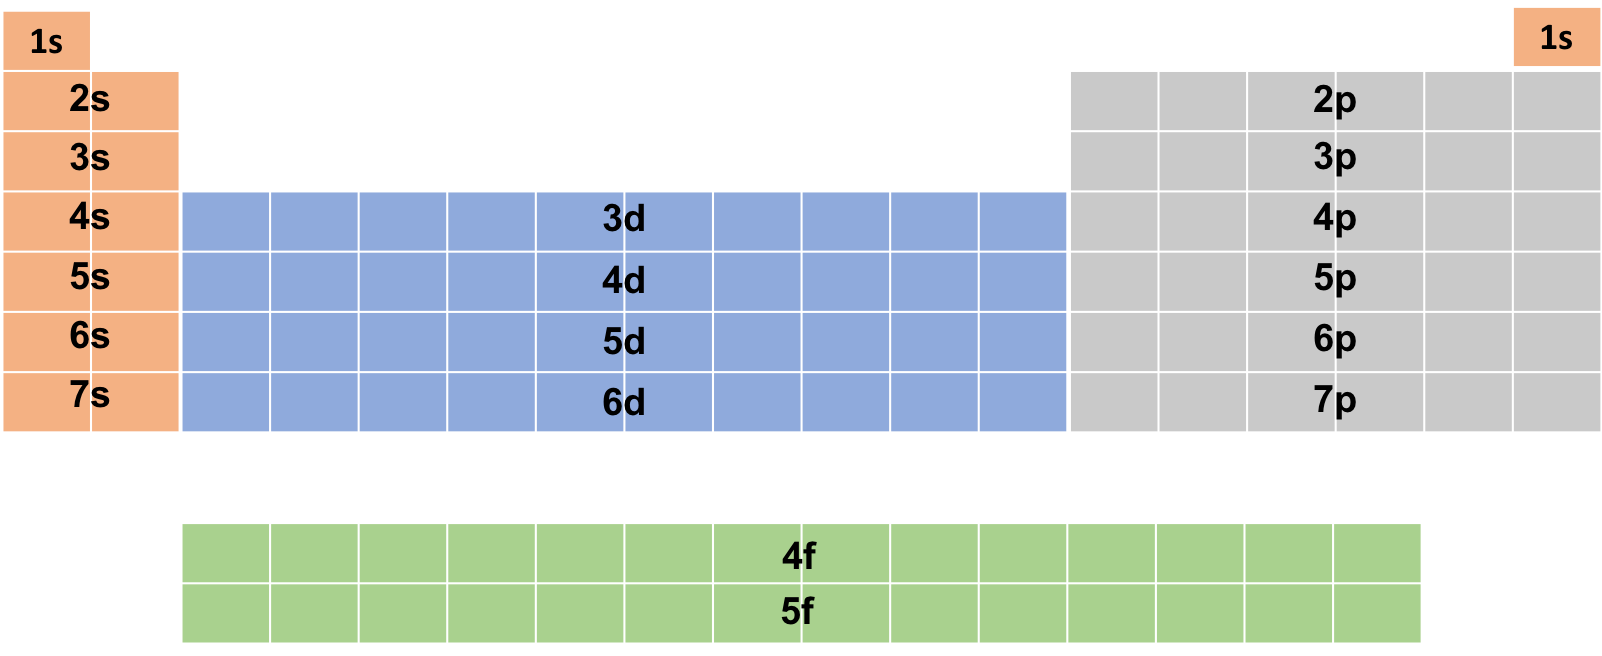
\includegraphics[scale=0.4]{aufbau_principle_2}
\end{center}

\subsubsection{Hund's Rule}

\begin{itemize}
    \item Due to electron-electron repulsion, electrons will fill orbitals of the same energy singly before pairing up.
\end{itemize}

\subsubsection{Pauli Exclusion Principle}

\begin{itemize}
    \item No two electrons in an atom will have the same set of 4 quantum numbers.
\end{itemize}

\subsection{Electron Configurations}

\subsubsection{Electron Configurations of Elements}

\begin{itemize}
    \item Fill with Aufbau principle.
    \item $1s^2 2s^2 2p^6 ...$
    \item Shorthand notation: write the name of the previous noble gas in square brackets, and then the rest of the electron configuration.
    \item Exceptions: \ce{Cr, Cu, Mo, Ag, Au} (Elements in group 6 and 11). Electron configuration is a half filled $s$ sub-shell and a half or fully filled $d$ sub-shell.
\end{itemize}

\subsubsection{Electron Configurations of Ions of Main Group Elements}

\begin{itemize}
    \item Write out the electron configuration of the neutral element.
    \item For anions: add electrons according to the Aufbau principle.
    \item For cations: remove electrons from the highest $n$ level and highest energy sub-shell.
    \item Isoelectronic: same number of electrons and same electron configuration.
    \item Most stable ions of atoms are isoelectronic with noble gases or have filled shells.
\end{itemize}

\subsubsection{Electron Configurations of Ions of Transition Elements}

\begin{itemize}
    \item Transition metals can lose both $n$ and $n-1$ valence electrons, but $n$ electrons are always lost first.
\end{itemize}

\subsubsection{Diamagnetic vs Paramagnetic Electron Configurations}

\begin{itemize}
    \item Diamagnetic: all electrons are paired. Will be repelled from externally produced magnetic fields.
    \item Paramagnetic: at least one electron is unpaired. Will be attracted to externally produced magnetic fields.
\end{itemize}

\section{Periodic Table Trends}

\subsection{Effective Nuclear Charge}

\begin{itemize}
    \item Inner electrons shield the outer electrons from the attractive force of the nucleus.
    \[Z_{eff} = Z - S\]
    \begin{itemize}
        \item $Z_{eff}$: effective nuclear charge
        \item $Z$: atomic number
        \item $S$: number of shielding electrons 
    \end{itemize}
    \item As we move to the right, $Z_{eff}$ increases. $Z$ increases and $S$ stays the same.
    \item As we move down a group, $Z_{eff}$ decreases. $S$ increases, more shielding.
\end{itemize}

\subsection{Atomic Radius}

\begin{itemize}
    \item Atomic radius: estimated radius from the nucleus to the outermost valence electrons.
    \item As we move to the right, $Z_{eff}$ increases, and the atomic radius decreases. 
    \item As we move down a group, $Z_{eff}$ decreases, and the atomic radius increases.
\end{itemize}

\subsubsection{Ranking Sizes: Ionic Radius}

\begin{itemize}
    \item Same element different charge: anions bigger, cations smaller.
    \item Different element same charge: identical trends to neutral atoms.
    \item Different element different charge:
    \begin{itemize}
        \item Can only be assessed for isoelectronic species.
        \item More protons: smaller radius.
        \item Less protons: greater radius.
    \end{itemize}
\end{itemize}

\subsection{Ionization Energy}

\begin{itemize}
    \item Ionization energy: the amount of energy required to remove the outermost electron in the gaseous phase.
    \item \ce{E -> E+ + e-}, $\Delta E =$ Ionization Energy ($IE$).
    \item As we move to the right, $Z_{eff}$ increases, ionization energy increases.
    \item As we move down a group, $Z_{eff}$ decreases, ionization energy decreases. 
\end{itemize}

\subsubsection{Comparing Ionization Energies}

\begin{align*}
    IE_1: &\ce{A(g) -> A+(g) + e-} \\
    IE_2: &\ce{A+(g) -> A2+(g) + e-} \\
    IE_3: &\ce{A2+(g) -> A3+(g) + e-} \\
\end{align*}
    
\begin{itemize}
    \item $IE_1 < IE_2 < IE_3 < IE_4 ...$
    \item To remove a core electron, ionization energy becomes much higher.
\end{itemize}

\subsection{Electron Affinity}

\begin{itemize}
    \item Electron affinity: the amount of energy involved with adding an electron.
    \item \ce{E + e- -> E-}, $\Delta E =$ Electron Affinity ($EA$).
    \item $EA$ is negative means energy is released and the atom is more stable with the electron added.
    \item $EA$ is positive means energy is absorbed and the atom is less stable with the electron added.
    \item Unless otherwise stated, use a negative $EA$ as a reference point (A negative $EA$ is greater).
    \item As $Z_{eff}$ increases, electron affinity increases. (This trend excludes noble gases).
\end{itemize}

\subsection{Electronegativity}

\begin{itemize}
    \item Electronegativity: a measure of electron pull. More electronegative elements will be more greedy for electrons.
    \item Electronegativity increases going up and to the right.
    \item General electronegativity order: F $>$ O $>$ N $>$ Cl $>$ Br $>$ I $>$ S $>$ C $\approx$ H
\end{itemize}

\begin{center}
    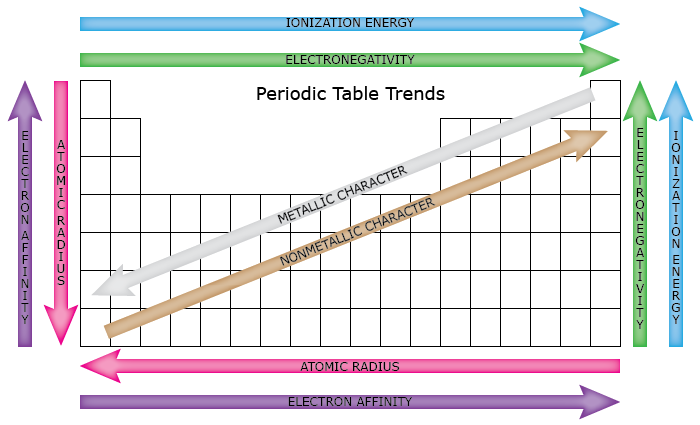
\includegraphics[scale=0.45]{periodic_table_trends.png}
\end{center}

\section{Chemical Bonding}

\subsection{Intramolecular Bonds}

\begin{itemize}
    \item Intramolecular bond: a bond that connects two atoms within a molecule together.
    \item Electronegativity: the tendency of an atom to pull bonding electrons towards itself.
    \item Increase in electronegativity difference: Non-polar Covalent bond $\rightarrow$ Polar Covalent Bond $\rightarrow$ Ionic Bond.
\end{itemize}

\subsection{Ionic Bonds}

\begin{itemize}
    \item Between a metal and a non-metal.
    \item Ionic compounds can be called salts.
    \item Large difference in electronegativity: $\Delta EN > 1.7$.
    \item The metal gives electrons to the non-metal.
\end{itemize}

\subsection{Covalent Bonds}

\begin{itemize}
    \item Between two non-metals.
    \item Electrons are shared.
\end{itemize}

\subsubsection{Non-polar Covalent Bonds}

\begin{itemize}
    \item Electrons are shared equally between 2 (often the same) non-metals.
    \item Small difference in electronegativity: $0 < \Delta EN < 0.4$.
\end{itemize}

\subsubsection{Polar Covalent Bonds}

\begin{itemize}
    \item Electrons are shared unequally between 2 different non-metals.
    \item Difference in electronegativity: $0.4 < \Delta EN < 1.7$.
    \item There is a vector dipole moment.
    \begin{itemize}
        \item Partial negative charge ($\delta -$) is assigned to atom with higher EN.
        \item Partial positive charge ($\delta +$) is assigned to atom with lower EN.
    \end{itemize}
\end{itemize}

\begin{center}
    \chemfig{
        \chemabove[3pt]{H}{\delta +}(-[::270,0.5,,,draw=none]@{a})-
        \chemabove[3pt]{Cl}{\delta -}(-[::270,0.5,,,draw=none]@{b})
    }
    \chemmove{
        \draw[____|-CF, thick] (a)--(b);
    }     
\end{center}

\subsubsection{Coordination Covalent Bonds}

\begin{itemize}
    \item Both electrons are donated by one of the nonmetals.
    \item The product can weakly conduct electricity in a solution.
\end{itemize}

\subsection{Properties of Covalent Bonds}

\subsubsection{Bond Length}

\begin{itemize}
    \item Bond length: the distance between two nuclei that are bound together when they are at their lowest possible energy state.
\end{itemize}

\subsubsection{Bond Dissociation Energy}

\begin{itemize}
    \item Bond dissociation energy: the amount of energy needed to break a bond homolytically.
    \item Breaking bonds will require energy, the higher the bond dissociation energy the stronger the bond.
\end{itemize}

\subsubsection{Bond Order}

\begin{itemize}
    \item The number of bonds between adjacent atoms.
    \item \ce{H-F}: single bond, bond order = 1.
    \item \ce{C=O}: double bond, bond order = 2.
    \item \ce{C#C}: triple bond, bond order = 3.
\end{itemize}

\subsubsection{Relationship}

\begin{itemize}
    \item For bonds between the same elements, the higher the bond order the bond length and the stronger the bond (higher bond dissociation energy)
\end{itemize}

\subsection{Metallic Bond}

\begin{itemize}
    \item Metal nucleus and inner shell electrons are surrounded by a sea of electrons.
    \item Conduction electrons are free to move around and are delocalized.
    \item Gives metal their properties: ductile, malleable, conduct thermal energy, conduct electricity, lustre/shine.
\end{itemize}

\section{Lewis Structures and Resonance Structures}

\subsection{Drawing Lewis Structures}

\begin{enumerate}
    \item Calculate the total number of valence electrons for the molecule.
    \item Write out all the atoms, with the central atom (usually the least electronegative) in the middle.
    \item Connect all atoms with single bonds.
    \item Put lone pairs on atoms, except \ce{H}, until there are no more electrons. Put extra lone pairs on the central atom.
    \item Shift lone pairs to make double or triple bonds to satisfy the Octet Rule and get the best formal charges.
\end{enumerate}

\begin{itemize}
    \item Octet rule: atoms tend to bond to have 8 valence electrons.
    \item Formal charges: the best Lewis Structure will have the lowest possible formal charge, with 0 being best.
\[FC = V - N - \frac{B}{2}\]
    \begin{itemize}
        \item $FC$: formal charge of the atom
        \item $V$: number of valence electrons
        \item $N$: number of non-bonding valence electrons
        \item $B$: total number of electrons shared in bonds
        \item If the formal charge is not zero, consider assigning negative formal charge to more electronegative elements, if possible.
    \end{itemize}
\end{itemize}

\subsubsection{Exceptions to the Octet Rule}

\begin{itemize}
    \item Octet deficient elements: less than 8 electrons.
    \begin{itemize}
        \item \ce{H} and \ce{He} can only have 2 electrons.
        \item \ce{Be} can only have 4 electrons.
        \item \ce{Al} and \ce{B} can only have 6 electrons.
    \end{itemize}
    \item Expanded octet elements: more than 8 electrons.
    \begin{itemize}
        \item \ce{P} can have 10 electrons.
        \item \ce{S} can have 12 electrons.
    \end{itemize}
    \item Radicals: odd number of electrons, unpaired electron makes it short-lived and highly reactive.
\end{itemize}

\subsubsection{Lewis Structures of Organize Compounds}

\begin{itemize}
    \item Carbon will usually be the central atoms.
    \item Carbon will form four bonds.
    \item Add lone pairs and shift them to satisfy Octet Rule.
    \item Example: \ce{CH3CH2CN} would be drawn as:
    \begin{center}
        \chemfig[atom sep=2em]{H-C(-[6]H)(-[2]H)-C(-[6]H)(-[2]H)-C~\Charge{0=\:}{N}}
    \end{center}
    \item Example: \ce{NH2CH2CH2CO2-} would be drawn as:
    \begin{center}
        $\chemleft[\chemfig[atom sep=2em]{\Charge{180=\:}{N}(-[:120]H)(-[:240]H)-C(-[2]H)(-[6]H)-C(-[2]H)(-[6]H)-C(-[:-60]\Charge{0=\:,180=\:,270=\:}{O})(=[:60]\Charge{0=\:,180=\:}{O})}\chemright]^{-}$
    \end{center}
    \item Example: \ce{CH3CH2NO2} would be drawn as:
    \begin{center}
        \chemfig[atom sep=2em]{H-C(-[2]H)(-[6]H)-C(-[2]H)(-[6]H)-N(-[:60]\Charge{0=\:,90=\:,270=\:}{O})(=[:-60]\Charge{0=\:,-120=\:}{O})}
    \end{center}
\end{itemize}

\subsubsection{Benzene Derivatives}

\begin{itemize}
    \item Benzene: 6 carbon ring with 3 double bonds. The double bonds are in resonance and can move around the ring.
    \item Example: p-aminosalicyclic acid (\ce{C7H7NO3}) would be drawn as:
    \begin{center}
        \chemfig[atom sep=2em]{\Charge{-150=\:}{N}(-[6]H)(-[:150]H)-[:30]C*6(-C(-[6]H)=C(-[:-30]H)-C(-[:30]C(-[2]\Charge{0=\:,90=\:,180=\:}{O})=[:-30]\Charge{270=\:}{O}-[:30]H)=C(-[2]\Charge{-30=\:,60=\:}{O}-[:150]H)-C(-[:150]H)=)}
    \end{center}
\end{itemize}

\subsection{Resonance Structures}

\begin{itemize}
    \item Resonance structures: used to describe molecules with delocalized electrons which cannot be described by a single Lewis structure.
    \item Resonance structures follow the same rules as Lewis structures.
    \item Move lone pairs and double bonds in a Lewis structure around to spread out the charge.
    \item Resonance hybrid: the "average" of all of a molecule's resonance structures. Consider the average bond order.
    \item Equivalent resonance structures: equally stable.
    \item Non-equivalent resonance structures: some are better than others.
    \begin{itemize}
        \item The major contributor (best resonance structure) will tend to have the smallest formal charges, and the negative charge resides on the more electronegative elements.
    \end{itemize}
\end{itemize}

\section{VSEPR Shapes and Polarity}

\subsection{VSEPR}

\begin{itemize}
    \item VSEPR (Valence Shell Electron Pair Repulsion theory): electron pairs in the valence shell dictates the molecular geometry.
\end{itemize}

\subsubsection{Electron Geometry}

\begin{itemize}
    \item Based on the central atom
\[EG = l + n\]
    \item $EG$: number of electron groups
    \item $l$: number of lone pairs 
    \item $n$: number of bound atoms to the central atom
\end{itemize}

\subsubsection{Molecular Geometry Table}

\begin{center}
    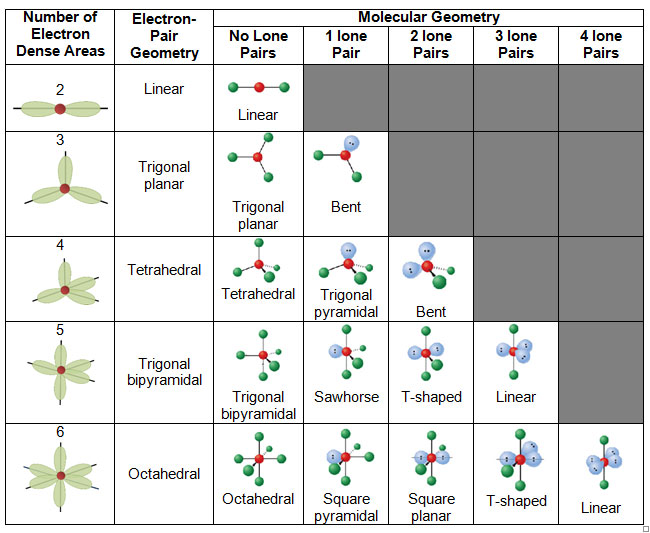
\includegraphics[scale=0.5]{vsepr.jpg}
\end{center}

\subsection{Molecular Polarity}

\begin{itemize}
    \item If there are no polar bonds, the molecule is non-polar.
    \item If there are polar bonds but they are symmetrical, the molecule is non-polar.
    \item If there are polar bonds that are not symmetrical, there is a net dipole moment and the molecule is polar.
\end{itemize}


\section{Intermolecular Forces and Physical Properties}

\begin{itemize}
    \item Intramolecular forces: forces acting between atoms within a molecular. Strong forces, such as covalent and ionic bonding.
    \item Intermolecular forces: attractive forces acting between molecules that are relatively weak.
\end{itemize}

\textbf{Intermolecular Forces}

\begin{itemize}
    \item Intermolecular forces are electrostatic in nature.
    \item Three main types:
    \begin{itemize}
        \item Hydrogen bonding.
        \item Dipole-Dipole bonding.
        \item London Dispersion Forces/Van der Waals forces.
    \end{itemize}
    \item Intermolecular forces are broken by physical changes.
    \item Intermolecular forces define physical properties of compounds (boiling points, melting points, solubility, vapour pressure, viscosities, etc.)
    \begin{itemize}
        \item The stronger the intermolecular forces, the higher the boiling and melting points.
    \end{itemize}
\end{itemize}

\subsubsection{Hydrogen Bonding}

\begin{itemize}
    \item Strongest intermolecular force.
    \item A \ce{H} from \ce{H-F}, \ce{H-O}, or \ce{H-N} bond interacts with a lone pair of electrons from another \ce{F}, \ce{O}, or \ce{N} atom. 
    \begin{itemize}
        \item The $\delta-$ on the electronegative atom attracts the $\delta+$ on the hydrogen atom that is bound to a highly electronegative atom (\ce{N}, \ce{O}, or \ce{F}).
        \item A hydrogen bond that involves \ce{F} will be the strongest, \ce{O} will be the second strongest, and \ce{N} will be the third strongest.
    \end{itemize}
    \item More hydrogen bonds implies higher boiling point.
\end{itemize}

\subsubsection{Dipole-Dipole Interactions}

\begin{itemize}
    \item Second strongest intermolecular force.
    \item The positive end of one polar molecule interacts with the negative end of another polar molecule.
\end{itemize}

\subsubsection{London Dispersion Forces/Van der Walls Forces}

\begin{itemize}
    \item Weakest intermolecular force.
    \item Interactions between temporary instantaneous dipoles that occur as electrons move around.
    \item London Dispersion Force is the interaction between two molecules with instantaneous dipoles.
    \item All substances can have London Dispersion Forces.
\end{itemize}

\subsection{Physical Properties}

\subsubsection{Phases}

\begin{itemize}
    \item Solids:
    \begin{itemize}
        \item Does not take the volume or shape of the container.
        \item Are not fluids.
        \item Has the strongest intermolecular forces.
    \end{itemize}
    \item Liquids:
    \begin{itemize}
        \item Does not fill the volume, but fills the shape, of the container.
        \item Are fluids.
        \item Has the weaker intermolecular forces.
    \end{itemize}
    \item Gases:
    \begin{itemize}
        \item Fills the volume and shape of the container.
        \item Are fluids.
        \item Has the weakest intermolecular forces.
    \end{itemize}
\end{itemize}

\subsubsection{Boiling and Melting Points}

\begin{itemize}
    \item Generally, a molecule with stronger intermolecular forces will have a higher boiling/melting point.
    \item When two molecules have the same type of intermolecular forces, the larger molecule based on molecular weight will have a higher boiling/melting point due to increased London Dispersion Forces.
    \item When two molecules have the same molecular weight, molecules with branched chains is easier to break apart and have lower boiling/melting points than molecules with linear chains. 
\end{itemize}

\subsubsection{Solubility}

\begin{itemize}
    \item Polar molecules are soluble in polar molecules, but are not soluble in non-polar molecules.
    \item Non-polar molecules are soluble in non-polar molecules, but are not soluble in polar molecules.
\end{itemize}

\subsubsection{Vapor Pressure}

\begin{itemize}
    \item Vapor pressure: pressure exerted by the gaseous phase of a liquid that evaporated from the exposed surface of a liquid.
    \item Molecules with lower intermolecular forces have higher vapor pressures. 
    \item Liquids with high vapor pressures are called volatile.
    \item As temperature increases, vapor pressure increases.
\end{itemize}

\section{Solids, Polymers, Phase Transitions \& Phase Diagrams}

\subsection{Solids}

\begin{itemize}
    \item Solids: one of the states of matter and are typically rigid.
\end{itemize}

\subsection{Polymers}

\begin{itemize}
    \item Polymers: a class of solids characterized by long chains of covalently linked atoms with a defined repeat unit.
    \item Made from a repeating monomer and usually have high molecular weight.
    \item Tend to form plastics or elastomers.
    \begin{itemize}
        \item Plastic: a material that can be changed into a new shape.
        \item Thermoplastic: a material that can be repeatedly reshaped.
        \item Thermosets: a plastic that cannot be reshaped.
        \item Elastomers: a material that exhibit elastic or rubbery behavior.
    \end{itemize}
    \item Tacticity: the relative arrangement of adjacent groups on a polymer chain.
    \begin{itemize}
        \item Isotactic: same side.
        \item Syndiotactic: alternating sides.
        \item Atactic: random. 
    \end{itemize}
    \item Tacticity can influence physical properties of the polymer.
    \begin{itemize}
        \item Polymers with high degree of isotacticity or syndiotacticity tend to have higher melting points.
    \end{itemize}
\end{itemize}

\subsubsection{Polymerization Reactions}

\begin{itemize}
    \item Addition polymerization:
    \begin{itemize}
        \item Monomer repeating unit is coupled with another monomer.
        \item The monomer unit usually has a double bond that breaks apart to form a chain of single bonds.
        \item Initiation, propagation, termination.
        \item Double bond becomes two single bonds. Example:
        \item Monomer: \chemfig[atom sep=2em]{=[:30]-[:90]*6(-=-=-=)}
        \item Polymer: \chemfig[atom sep=2em]{-[:30,1.5](-[:90]*6(-=-=-=))-[:-30,1.5]-[:30,1.5](-[:90]*6(-=-=-=))-[:-30,1.5]-[:30,1.5](-[:90]*6(-=-=-=))-[:-30,1.5]}
        \item Polyethylene (PE): \chemfig[atom sep=2em]{-[@{left,0.5}]C(-[2]H)(-[6]H)-C(-[2]H)(-[6]H)-[@{right,0.5}]}
        % \polymerdelim[delimiters={[]}, height=22pt, depth=, indice=n]{left}{right}
        % For some reason this is not working in vscode latex but it works in overleaf
        \item Polypropylene (PP): \chemfig[atom sep=2em]{-[@{left,0.5}]C(-[2]H)(-[6]CH_3)-[,1.5]C(-[2]H)(-[6]H)-[@{right,0.5}]}
        % \polymerdelim[delimiters={[]}, height=22pt, depth=, indice=n]{left}{right}
        \item Polystyrene (PS): \chemfig[atom sep=2em]{-[@{left,0.5},2]C(-[2]*6(=-=-=-))(-[6]H)-C(-[2]H)(-[6]H)-[@{right,0.5}]}
        % \polymerdelim[delimiters={[]}, height=60pt, depth=22pt, indice=n]{left}{right}
        \item Polyvinylchloride (PVC): \chemfig[atom sep=2em]{-[@{left,0.5}]C(-[2]H)(-[6]H)-C(-[2]H)(-[6]Cl)-[@{right,0.5}]}
        % \polymerdelim[delimiters={[]}, height=22pt, depth=, indice=n]{left}{right}
    \end{itemize}
    \item Condensation polymerization:
    \begin{itemize}
        \item Two different monomer units are joined to form a polymer and a small molecule is eliminated.
    \end{itemize}
\end{itemize}

\subsection{Phase Changes}

\begin{itemize}
    \item Melting: solid to liquid. Freezing: liquid to solid.
    \item Vaporization: liquid to gas. Condensation: gas to liquid.
    \item Sublimation: solid to gas. Deposition: gas to solid.
    \item Terminology:
    \begin{itemize}
        \item Melting = fusion.
        \item Freezing = crystallization.
        \item Boiling = vaporization.
    \end{itemize}
    \item Endothermic: $\Delta H > 0$, heat is added.
    \item Exothermic: $\Delta H < 0$, heat is released.
\end{itemize}

\subsection{Phase Diagrams}

\begin{itemize}
    \item A plot of pressure vs temperature.
    \item Triple point: where solid, liquid, and gas are at equilibrium.
    \item Critical Point: the point at which liquid and gas are indistinguishable.
    \item Supercritical fluid: matter which has been pushed to temperatures and pressures beyond its critical point.
    \item For most compounds, the melting curve has a positive slope. Uncommonly, the melting curve for some compounds (such as water) has a negative slope. The liquid form of these compounds are more dense than their solid form.
\end{itemize}

\begin{center}
    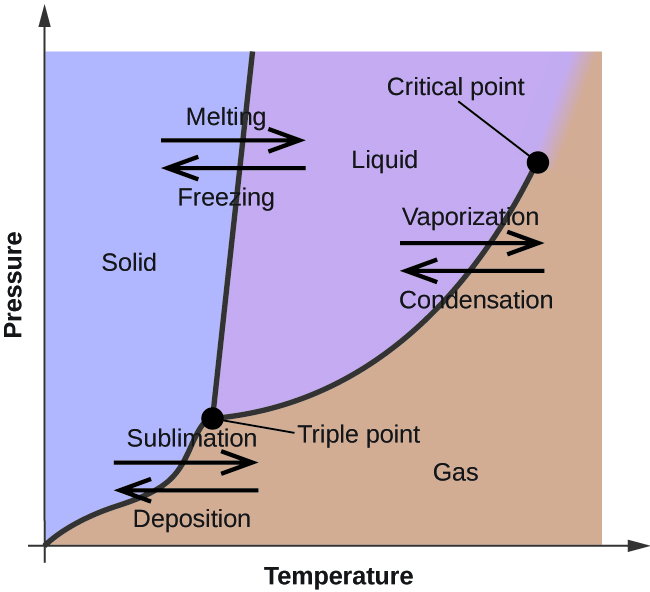
\includegraphics[scale=0.5]{phase_diagram.jpg}
\end{center}

\section{Gases and Their Properties}

\subsection{Ideal Gas}

\begin{itemize}
    \item Ideal gases have negligible volume and no intermolecular forces.
\end{itemize}

\subsubsection{Ideal Gas Law}

\begin{equation*}
    PV=nRT
\end{equation*}

\begin{itemize}
    \item P: pressure in \si{\pascal} or \si{\kilo\pascal} or \si{\bar} or \si{\atm} or \si{\mmHg} or \si{torr}
    \item V: volume in \si{\litre} or \si{\meter\cubed}
    \item n: amount of substance in \si{\mole}
    \item R: ideal gas constant = \SI[per-mode = fraction]{8.3145}{\joule\per\mole\per\kelvin} = \SI[per-mode = fraction]{8.3145}{\kilo\pascal\litre\per\mole\per\kelvin} = \SI[per-mode = fraction]{0.08206}{\atm\litre\per\mole\per\kelvin}
    \item T: temperature in \si{\kelvin}
\end{itemize}

\subsubsection{Gas Laws}

\begin{center}
    \renewcommand{\arraystretch}{2}
    \begin{tabular}{|c|c|c|}
        \hline
        Name & Conditions & Equation \\
        \hline 
        Boyle's Law & Constant $T$ and $n$ & $P_1V_1 = P_2V_2$ \\
        \hline
        Charles' Law & Constant $P$ and $n$ & $\frac{V_1}{T_1} = \frac{V_2}{T_2}$ \\
        \hline
        Gay Lussac's Law & Constant $V$ and $n$ & $\frac{P_1}{T_1} = \frac{P_2}{T_2}$ \\
        \hline
        Avogradro's Law & Constant $P$ and $T$ & $\frac{V_1}{n_1} = \frac{V_2}{n_2}$ \\
        \hline
        Combined Gas law & Constant $n$ & $\frac{P_1V_1}{T_1} = \frac{P_2V_2}{T_2}$ \\
        \hline
    \end{tabular}
\end{center}

\subsubsection{Standard Molar Volume}

\begin{itemize}
    \item At STP (standard temperature and pressure) where $P$ = \SI{1}{\atm} and $T$ = \SI{0}{\celsius} = \SI{273.15}{\kelvin}, \SI{1}{\mole} of any gas occupies \SI{22.4}{\litre}.
\end{itemize}

\subsection{Real Gas}

\begin{itemize}
    \item Real gases have volume and have intermolecular forces.
    \item Real gases act most like ideal gases when temperature is high and pressure is low.
    \item In a constant pressure container:
    \begin{itemize}
        \item For real gases, volume of the container is less than that for ideal gases.
    \end{itemize}
    \item In a constant volume container:
    \begin{itemize}
        \item For real gases, pressure of the container is less than that for ideal gases.
    \end{itemize}
\end{itemize}

\subsubsection{Van der Waals Equation}

\begin{equation*}
    \left(P + a\frac{n^2}{V^2}\right)(V - nb) = nRT
\end{equation*}

\begin{itemize}
    \item $a$: attractive force correction.
    \begin{itemize}
        \item $a$ increases with increasing intermolecular attraction between gas molecules.
    \end{itemize}
    \item $b$: bulkiness correction.
    \begin{itemize}
        \item $b$ increases with molecular weight of gas molecules.
    \end{itemize}
    \item $a$ and $b$ are experimentally determined.
\end{itemize}

\subsubsection{Compressibility Factor}

\begin{equation*}
    Z = \frac{PV}{RT}
\end{equation*}

\begin{itemize}
    \item Z: compressibility factor
    \item V: molar volume in \si[per-mode = fraction]{\litre\per\mole}
    \item For an ideal gas, $Z = 1$.
\end{itemize}

\subsection{Gas Mixtures and Partial Pressures}

\subsubsection{Total Pressure}

\begin{equation*}
    P_{total} = P_1 + P_2 + P_3 \dots = \sum P_i
\end{equation*}

\begin{equation*}
    P_{total} = \frac{n_{total} RT}{V}
\end{equation*}

\begin{itemize}
    \item $P_{total}$: the measured pressure of the mixture
    \item $P_i$: the partial pressure of gas $i$
    \item Partial pressure: the pressure that would be exerted by one of the gases in the mixture if it occupied the same volume on its own.
    \item The total pressure depends only on the total moles of gas, and not the identity of the gases.
\end{itemize}

\subsubsection{Partial Pressure}

\begin{equation*}
    P_A = \frac{n_A}{n_{total}} P_{total} = X_A P_{total}
\end{equation*}

\begin{itemize}
    \item $P_A$: partial pressure of gas $A$
    \item $X_A$: mole fraction of gas $A$
\end{itemize}

\subsection{Kinetic Molecular Theory (KMT)}

\subsubsection{Assumptions of KMT}

\begin{itemize}
    \item Ideal gases are in constant, random motion and move in straight lines.
    \item Volume is considered to be $0$.
    \item Collisions are completely elastic.
    \item There are no intermolecular forces.
    \item Temperature is directly proportional to the average kinetic energy.
\end{itemize}

\subsubsection{Kinetic Energy, Temperature, and Speeds}

\begin{itemize}
    \item Average kinetic energy of a gas:
\end{itemize}    

\begin{equation*}
    KE_{avg} = \frac{3}{2}RT
\end{equation*}

\begin{itemize}
    \item[] \begin{itemize}
        \item R: ideal gas constant = \SI[per-mode = fraction]{8.3145}{\joule\per\mole\per\kelvin}
        \item T: temperature in \si{\kelvin}
    \end{itemize}
    \item Speed of gas particles in one container:
    \begin{itemize}
        \item Speed is distributed according to the Maxwell-Boltzmann distribution.
        \item The higher the temperature, the broader the speed distribution
    \end{itemize}
    \item Average speed of two different gases at the same temperature:
    \begin{itemize}
        \item Same kinetic energy $\implies$ heavier gases will have a slower average speed than lighter gases.
        \item Lighter gases have a broader speed distribution.
    \end{itemize}
    \item Root Mean Squared Speed:
\end{itemize}

\begin{equation*}
    u_{rms} = \sqrt{\frac{3RT}{M}}
\end{equation*}

\begin{itemize}
    \item[] \begin{itemize}
        \item R: ideal gas constant = \SI[per-mode = fraction]{8.3145}{\joule\per\mole\per\kelvin}
        \item T: temperature in \si{\kelvin}
        \item M: molar mass in \si[per-mode = fraction]{\kilo\gram\per\mol}
    \end{itemize}
\end{itemize}

\subsection{Diffusion and Effusion}

\subsubsection{Diffusion}

\begin{itemize}
    \item Mixing molecules of one gas with another as a result of random molecular movement.
\end{itemize}

\subsubsection{Effusion}

\begin{itemize}
    \item Escape of gas molecules from their container through a tiny pinhole.
    \item Lighter molecules effuse faster.
    \item Graham's Law of Effusion:
\end{itemize}

\begin{equation*}
    \frac{r_A}{r_B} = \frac{(u_{rms})_A}{(u_{rms})_B} = \sqrt{\frac{M_B}{M_A}}
\end{equation*}

\begin{itemize}
    \item[] \begin{itemize}
        \item $r$: rate of effusion
        \item $M$: molar mass
    \end{itemize}
\end{itemize}

\section{Thermochemistry}

\subsection{Introduction}

\begin{center}
    \begin{tabular}{|c|c|} 
        \hline
        \textbf{Term} & \textbf{Definition} \\
        \hline
        System & The collection of matter under consideration \\
        \hline
        Surroundings & Everything not part of the system \\
        \hline
        Open System & Can exchange matter and energy with surroundings \\
        \hline
        Closed System & Can only exchange energy with surroundings \\
        \hline
        Isolated System & Cannot exchange matter or energy with surroundings \\
        \hline
    \end{tabular}
\end{center}

\begin{itemize}
    \item State variable: a variable that depends only on the current state of the system, independent of the path taken to get to that state.
    \item Extensive properties: depends on the amount of a substance.
    \item Intensive properties: does not depend on the amount of substance.
\end{itemize}

\subsection{\nth{0} Law of Thermodynamics}

\begin{itemize}
    \item If two bodies are both in thermal equilibrium with a third body, then they are also in thermal equilibrium with each other.
\end{itemize}

\subsection{\nth{1} Law of Thermodynamics}

\begin{itemize}
    \item The energy of an isolated system is constant.
    \begin{equation*}
        \Delta E = \Delta U = Q + W
    \end{equation*}
    \begin{itemize}
        \item $E$ = $U$: internal energy of a closed system
        \item $Q$: heat in \si{\joule}
        \item $W$: work in \si{\joule}
        \item Net energy transfers into the system is positive and net energy transfer from the system is negative.
        \item Internal energy of a closed system is only dependent on its temperature.
    \end{itemize}
    \item Calculating work for constant external pressure:
    \begin{equation*}
        W = -P \Delta V
    \end{equation*}
    \begin{itemize}
        \item $W$: work in \si{\joule}
        \item $P$: pressure in \si{\kilo\pascal}
        \item $V$: volume in \si{\litre}
    \end{itemize}
\end{itemize}

\subsection{Calorimetry}

\begin{itemize}
    \item Enthalpy: a state function which measures the heat flow of a reaction at constant pressure.
    \begin{equation*}
        H = E + PV
    \end{equation*}
    \begin{itemize}
        \item $H$: enthalpy
        \item $E$: internal energy
        \item $P$: pressure
        \item $V$: volume    
        \item $-\Delta H$ means an exothermic process.
        \item $+\Delta H$ means an endothermic process.
    \end{itemize}
    \item Heat Capacity:
    \begin{equation*}
        q = C \Delta T = n C_m \Delta T = m C_s \Delta T
    \end{equation*}
    \begin{itemize}
        \item $q$: heat in \si{\joule}
        \item $n$: amount of substance in \si{\mole}
        \item $m$: mass in \si{\gram}
        \item $C$: heat capacity in \si[per-mode = fraction]{\joule\per\celsius}
        \item $C_m$: molar heat capacity in \si[per-mode = fraction]{\joule\per\mole\per\celsius}
        \item $C_s$ (also written as $c$): specific heat in \si[per-mode = fraction]{\joule\per\gram\per\celsius} 
    \end{itemize}
    \item Calorimeters: an insulated container that usually holds water. 
    \begin{itemize}
        \item A thermometer measures the temperature of the water. 
        \item If the temperature of the water increases, then the reaction is exothermic. If the temperature of the water decreases, then the reaction is endothermic.
        \item Coffee cup calorimeter: pressure is constant.
        \item Bomb calorimeter: volume is constant.
    \end{itemize}
    \item Heat during a phase change:
    \begin{equation*}
        q = mL
    \end{equation*}
    \begin{itemize}
        \item $q$: heat in \si{\joule}
        \item $m$: mass
        \item $L$: specific latent heat
    \end{itemize}
    \item Heating curve:
    \begin{center}
        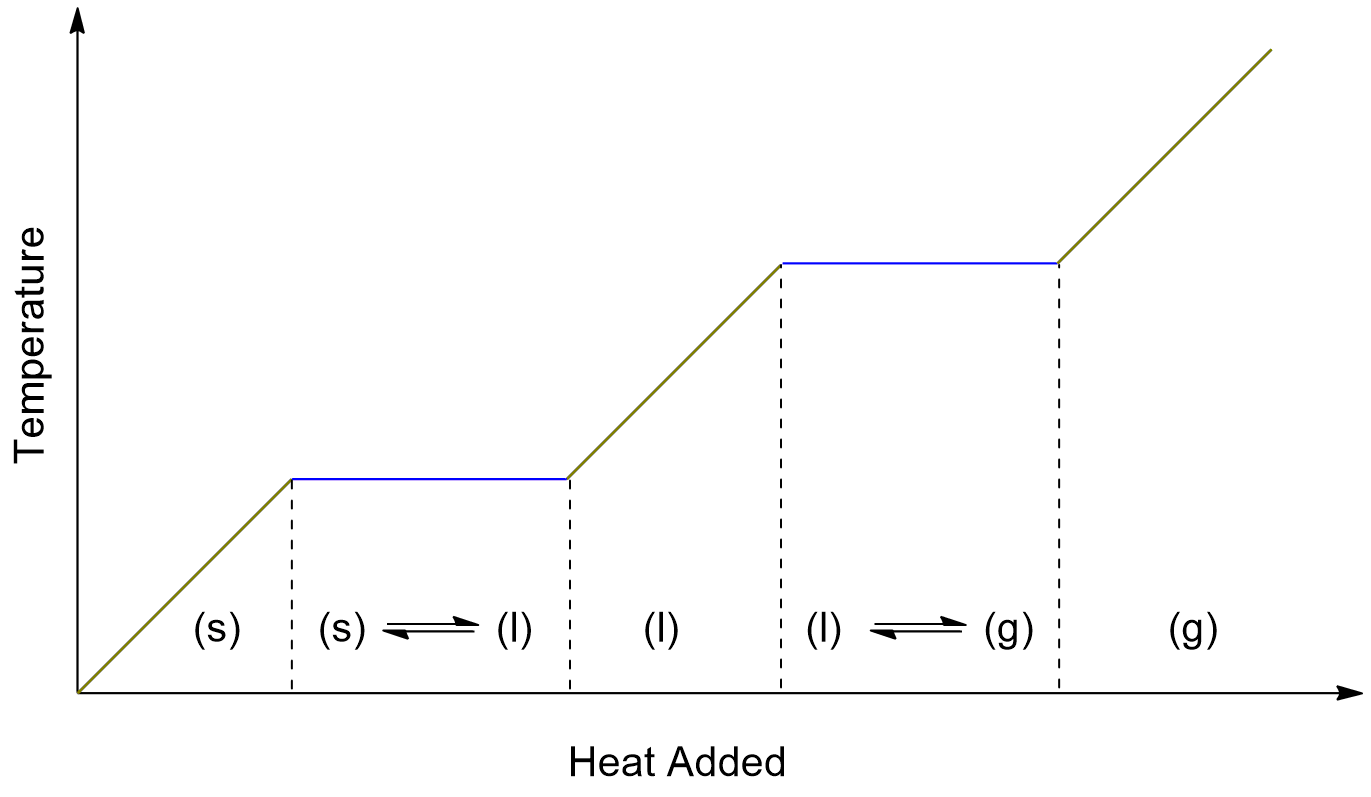
\includegraphics[scale = 0.3]{heating_curve.png}
    \end{center}
    \item Cooling curve:
    \begin{center}
        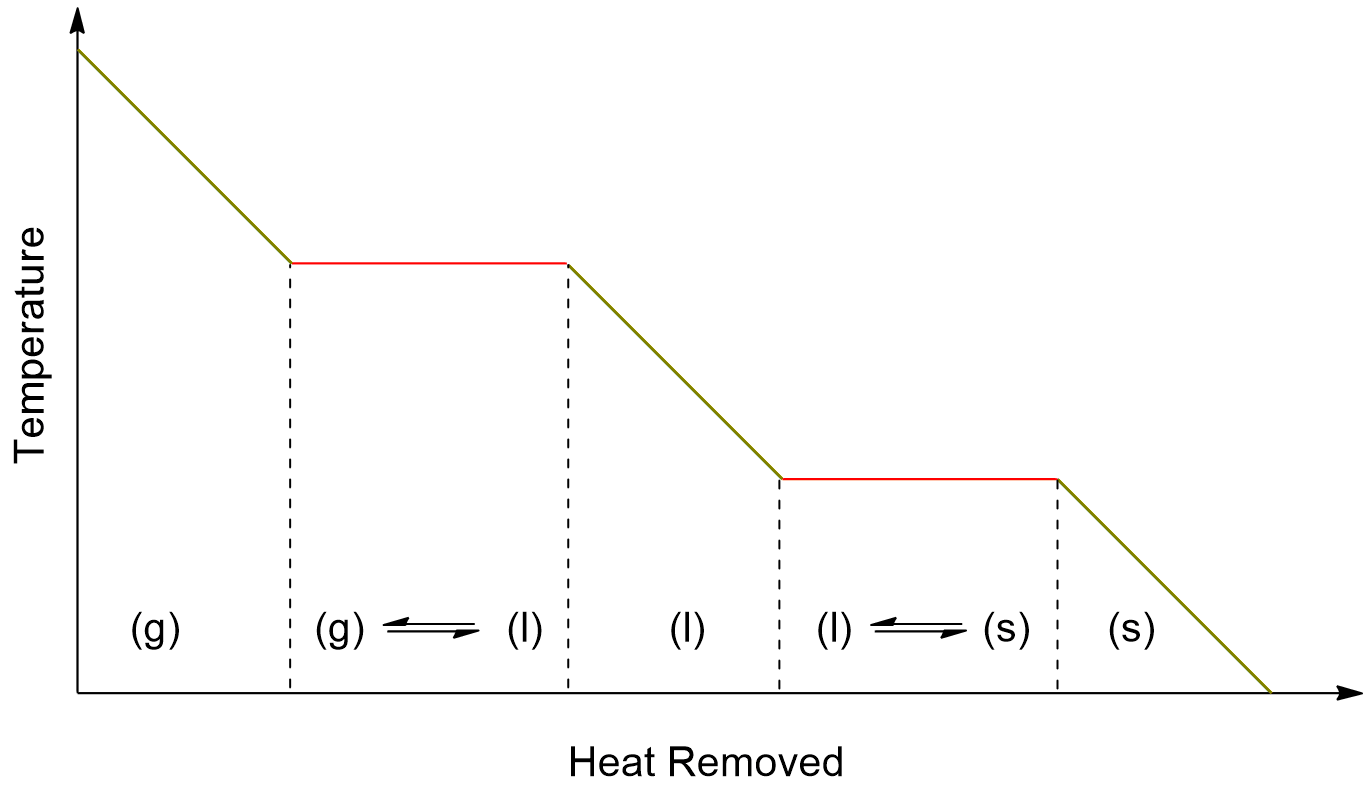
\includegraphics[scale = 0.3]{cooling_curve.png}     
    \end{center}
\end{itemize}

\subsection{Heat of Formation and Reaction}

\subsubsection{Heat of Formation}

\begin{itemize}
    \item Formation reaction: reactants are elements in their standard state, and there is only one mole of product.
    \item $\Delta H_{f}^\circ$: standard heat of formation in \si[per-mode = fraction]{\kilo\joule\per\mole}. 
    \item Standard heat of formation of any element is $0$. 
    \item $\Delta H^\circ$ of the reaction can be calculated from the $\Delta H_{f}^\circ$ of the chemicals, which can be looked up in a table.
\end{itemize}

\subsubsection{Heat of Reaction}

\begin{itemize}
    \item Standard heat of a reaction: $\Delta H^\circ$. The heat when the number of moles of chemicals specified in the balanced chemical equation reacts at standard state. Positive $\Delta H^\circ$ means heat is required, negative $\Delta H^\circ$ means heat is produced.
    \begin{equation*}
        \Delta H^\circ = \Sigma (\Delta H_f^\circ \times \text{coefficient})_{\text{products}} - \Sigma (\Delta H_f^\circ \times \text{coefficient})_{\text{reactants}}
    \end{equation*}
    \item When the reaction is no longer is standard state, the superscript $\circ$ is dropped.
    \item Hess's Law: when mathematical operations are performed on a chemical equation, the same mathematical operations are applied to the heat of reaction.
    \begin{itemize}
        \item If the coefficients are multiplied by a constant, $\Delta H^\circ$ is multiplied by the same constant.
        \item If multiple equations are added, the $\Delta H^\circ$ of the equations are also added to give the heat of the overall equation.
    \end{itemize}
    \item $\Delta H_{forward}^\circ = -\Delta H_{reverse}^\circ$.
\end{itemize}

\subsection{\nth{2} and \nth{3} Law of Thermodynamics}

\begin{itemize}
    \item Entropy ($S$): the state of disorder of a system, in \si[per-mode = fraction]{\joule\per\celsius}.
    \item \nth{2} Law of Thermodynamics: the entropy of an isolated system cannot decrease.
    \item \nth{3} Law of Thermodynamics: the entropy of a system approaches a constant value when its temperature approaches absolute zero.
    \item Statistical method for determining entropy: $S = k \ln w$.
    \begin{itemize}
        \item $k$: Boltzmann constant = \SI[per-mode = fraction]{1.380649e-23}{\joule\per\kelvin}
        \item $w$: number of microstates
    \end{itemize}
    \item Experimental method for determining entropy: $S^\circ = \frac{q_\text{rev}}{T}$.
    \begin{itemize}
        \item $S^\circ$: standard entropy, the entropy of one mole of a chemical at a temperature
        \item $q_\text{rev}$: the heat added to raise the temperature very slowly from absolute zero up to $T$
        \item $T$: temperature in \si{\kelvin}
    \end{itemize}
    \item Change in entropy during a chemical process:
    \begin{equation*}
        \Delta S^\circ = \Sigma (\Delta S_f^\circ \times \text{coefficient})_{\text{products}} - \Sigma (\Delta S_f^\circ \times \text{coefficient})_{\text{reactants}}
    \end{equation*}
    \item Estimating entropy:
    \begin{itemize}
        \item Formation of a gas increases entropy greatly.
        \item Changes from solid to liquid increases entropy.
        \item Increase in temperature increases entropy.
    \end{itemize}
\end{itemize}

\subsubsection{Predicting Spontaneity from Gibbs Free Energy}

\begin{itemize}
    \item Under constant temperature and pressure, the state function Gibbs Free Energy $\Delta G$ can predict whether a reaction is spontaneous.
    \begin{equation*}
        \Delta G = \Delta H - T \Delta S
    \end{equation*}
    \begin{itemize}
        \item $\Delta G$: Gibbs Free Energy in \si{\joule}
        \item $\Delta H$: enthalpy in \si{\joule}
        \item $T$: temperature in \si{\kelvin}
        \item $\Delta S$: entropy in \si[per-mode = fraction]{\joule\per\kelvin}
    \end{itemize}
    \item If $\Delta G > 0$, the reaction is non-spontaneous and the reverse reaction is spontaneous.
    \item If $\Delta G < 0$, the reaction is spontaneous and irreversible. 
\end{itemize}

\begin{center}
    \begin{tabular}{|c|c|c|c|}
        \hline $\Delta H^\circ$ & $\Delta S^\circ$ & $\Delta G^\circ$ as $T$ increases & Spontaneity \\
        \hline Negative & Positive & Always negative & Always spontaneous \\
        \hline Positive & Negative & Always positive & Always nonspontaneous \\
        \hline Negative & Negative & Becomes positive & Becomes nonspontaneous \\
        \hline Positive & Positive & Becomes negative & Becomes nonspontaneous \\
        \hline
    \end{tabular}
\end{center}

\subsubsection{Predicting Spontaneity from Entropy}

\begin{center}
    \begin{tabular}{|c|c|c|}
        \hline $\Delta S_\text{system}$ & $\Delta S_\text{surroundings}$ & Spontaneity \\
        \hline Positive & Positive & Spontaneous \\
        \hline Negative & Negative & Nonspontaneous \\
        \hline Negative & Positive & Depends on the magnitude \\
        \hline Positive & Negative & Depends on the magnitude \\
        \hline
    \end{tabular}
\end{center}

% \end{comment}

\section{Equilibrium}

\begin{itemize}
    \item Reactions reach an equilibrium when the rate of the forward reaction and reverse reaction are equal.
    \item Changes still occur on the microscopic level, but on the macroscopic level, the concentrations remain constant.
\end{itemize}

\subsection{The Equilibrium Constant $K$}

\begin{itemize}
    \item Represented by the symbol $K$. Subscripts indicate the type of equilibrium constant. 
\end{itemize}

\subsubsection{$K_c$}

\begin{itemize}
    \item When concentration is expressed in molarity, $K_c$ is used. 
    \item For a general reaction \ce{aA + bB <=> cC + dD}, $K_c = \dfrac{[C]^c [D]^d}{[A]^a [B]^b}$ when the reaction is at equilibrium.
    \begin{itemize}
        \item Example: For the reaction \ce{C3H8(g) + 5O2(g) <=> 3CO2(g) + 4H2O(g)}, $K_c = \dfrac{[\ce{CO2}]^3 [\ce{H2O}]^4}{[\ce{C3H8}] [\ce{O2}]^5}$. 
    \end{itemize}
    \item Liquids and solids are never included in the equilibrium expression.
    \item What the magnitude of $K_c$ indicates:
    \begin{itemize}
        \item $K_c > 1$: the reaction is thermodynamically favoured, and there are more products.
        \item $K_c = 1$: there are equal amounts of products and reactants.
        \item $K_c < 1$: the reaction is not thermodynamically favoured, and there are more reactants.
    \end{itemize}
    \item Manipulating the equilibrium constant:
    \begin{itemize}
        \item $K_c'$ for the reverse reaction is equal to $\dfrac{1}{K_c}$.
        \item $K_c'$ for the reaction where coefficients are multiplied by $C$ is equal to $(K_c)^C$.
        \item $K_c'$ for the sum of two reactions is equal to $K_1 K_2$.
    \end{itemize}
\end{itemize}

\subsubsection{$K_p$}

\begin{itemize}
    \item When partial pressures are involved, $K_p$ is used.
    \begin{equation*}
        K_p = K_c (RT)^{\Delta n}
    \end{equation*}
    \begin{itemize}
        \item $R$: ideal gas constant
        \item $T$: temperature in \si{\kelvin}
        \item $\Delta n$: moles of gas on products - moles of gas on reactants 
    \end{itemize}
    \item When given partial pressures, $K_p$ is calculated in the same way as $K_c$.
\end{itemize}

\subsection{The Reaction Quotient $Q$}

\begin{itemize}
    \item When the reaction is not in equilibrium, $Q = \dfrac{[C]^c [D]^d}{[A]^a [B]^b}$.
    \begin{itemize}
        \item If $Q = K_c$, the reaction is in equilibrium.
        \item If $Q < K_c$, the reaction will move in the forward direction (to the right) in order to achieve equilibrium.
        \item If $Q > K_c$, the reaction will move in the reverse direction (to the left) in order to achieve equilibrium. 
    \end{itemize}
\end{itemize}

\subsubsection{$K_{sp}$}


\begin{itemize}
    \item When solubility is involved, $K_{sp}$ is used.
    \item Calculated using the molar solubility of reagents at equilibrium.
    \item Solubility of Ionic Compounds at SATP
\end{itemize}

\begin{center}
    \resizebox{\textwidth}{!}{
    \begin{tabular}{|p{4em}|p{7em}|p{8em}|p{7em}|p{8em}|p{8em}|p{7em}|p{4em}|p{3em}|}
        \hline
         & & \multicolumn{7}{c|}{Anions} \\
        \hline & & \ce{Cl-}, \ce{Br-}, \ce{I-} & \ce{S2-} & \ce{OH-} & \ce{SO4^2-} & \ce{CO3^2-}, \ce{PO4^3-} & \ce{C2H3O2-} & \ce{NO3-} \\
        \hline \multirow{4}{*}{Cations} & High solubility $\ge$ \SI[per-mode=symbol]{0.1}{\mole\per\litre} & most & Group 1, Group 2, \ce{NH4+} & Group 1, \ce{NH4+}, \ce{Sr2+}, \ce{Ba2+}, \ce{Tl+} & most & Group 1, \ce{NH4+} & most & all \\
        \cline{2-9} & Low solubility $<$ \SI[per-mode=symbol]{0.1}{\mole\per\litre} & \ce{Ag+}, \ce{Pb2+}, \ce{Tl+}, \ce{Hg2^2+}, \ce{Cu+} & most & most & \ce{Ag+}, \ce{Pb2+}, \ce{Ca2+}, \ce{Ba2+}, \ce{Sr2+}, \ce{Ra2+} & most & \ce{Ag+} & none \\
        \hline
    \end{tabular}
    }
\end{center}

\begin{itemize}
    \item When a combination of ions is highly soluble, no precipitate will form.
    \item When a combination of ions has low solubility, a precipitate might form, but we must verify that $Q>K_{sp}$.
    \item Factors that affect solubility:
    \begin{itemize}
        \item Common ion effect: the solubility of a salt is reduced by the presence of another salt having a common ion.
        \item Complex ion formation: reactions that use up one of the ions, to form a complex ion, will increase the solubility of a salt.
        \item Acid-base neutralization: if the anion of the salt is the conjugate base of a weak acid, the solubility of the salt will increase in an acidic solution.
    \end{itemize}
\end{itemize}

\subsection{Le Chatelier's Principle}

\begin{itemize}
    \item Henry Le Chatelier's fundamental principle of chemical equilibrium, proposed in 1888.
    \item Whenever a system in dynamic equilibrium is disrupted, the system will respond to reestablish a new equilibrium state, if possible.
    \item Consequences of Le Chatelier's Principle:
    \begin{itemize}
        \item When the concentration of a reagent is increased, the reaction will shift towards the opposite side.
        \item When the pressure is increased, the reaction will shift towards the side with less moles of gas.
        \item When the volume is increased, the pressure decreases, the reaction will shift towards the side with more moles of gas. 
        \item When the heat is added, it depends on whether the reaction is endothermic or exothermic. We treat heat as a reagent, and consider adding heat as increasing the concentration of a reagent. 
    \end{itemize}
\end{itemize}

\subsection{ICE Tables}


\begin{itemize}
    \item Initial concentration, change in concentration, concentration at equilibrium. 
    \item Example usage of ICE table: At \SI{150}{\celsius}, $K_c$ for the reaction \ce{I2(g) + Br2(g) <=> 2IBr(g)} is \SI{1.20e2}{}. Starting with \SI{4}{\mole} each of iodine and bromine in a \SI{2}{\litre} flask, calculate the equilibrium concentrations of all reagents.
    \begin{center}
        \begin{tabular}{|c|c|c|c|}
            \hline Reaction & \ce{I2} & \ce{Br2} & \ce{IBr} \\
            \hline I & \SI{2}{\Molar} & \SI{2}{\Molar} & 0\\
            \hline C & $-x$ & $-x$ & $+2x$ \\
            \hline E & $2-x$ & $2-x$ & $2x$ \\
            \hline 
        \end{tabular}        
    \end{center}
    \item $K_c = \dfrac{[\ce{IBr}]^2}{[\ce{I2}][\ce{Br2}]} = \frac{(2x)^2}{(2-x)^2} = 1.20 \times 10^2$. Solving gives $x = 1.69$, so the concentrations of \ce{I2}, \ce{Br2}, and \ce{IBr} are \SI{0.309}{\Molar}, \SI{0.309}{\Molar}, and \SI{3.38}{\Molar} respectively.
\end{itemize}

\end{document}
